\chapter{Polarisation Spectroscopy}
\pagenumbering{arabic}
\setcounter{page}{1}

\section{Literature Review $\leftarrow$ rename at some point}

Laser frequency stabilisation is an essential tool for atomic physics experiments, without it experiments such as \gls{bec} and atomic clocks would not be possible~~\cite{anderson_observation_1995,ye_quantum_2008}.
There are a large number of techniques available for laser frequency stabilisation with numerous advantages and disadvantages among them.

\Gls{ps} is one such technique that will be discussed in detail here.
\Gls{ps} was first described by Wieman and H\"anch in 1976 as, ``We have demonstrated a sensitive new method of Doppler-free spectroscopy, monitoring the nonlinear interaction of two monochromatic laser beams in an absorbing gas via changes in light polarisation."\cite{wieman_doppler-free_1976}
A detailed discussion of physics of \gls{ps} can be found in Section \ref{section:pol_spec_theory}.

\subsection{Laser Frequency Stabilisation}

Laser frequency stabilisation describe a number of techniques that are used to reduce the temporal frequency spread of a lasers frequency.
Typically these techniques use some reference to measure frequency deviation from a given frequency and feedback to the laser.

Origin of freq noise.

How to control freq.

\subsubsection{from paper - merge}
The desirable traits of a laser frequency stabilization scheme include the ability to stabilize to an absolute atomic reference, absence of frequency or amplitude modulation, high bandwidth to achieve low spectral linewidth, low complexity and low cost.
Techniques for stabilization include \gls*{sa}~\cite{maguire_theoretical_2006, haroche_theory_1972, preston_doppler-free_1996}, which can reduce \gls*{ecdl} linewidth below 100\,kHz \cite{cuneo_optically_1994, saliba_linewidths_2009}, through to elaborate experiments involving extremely high-finesse optical cavities that are able to achieve sub-hertz linewidth using the \gls*{pdh} technique \cite{ludlow_compact_2007}.
Saturated absorption spectroscopy, \gls*{davll} \cite{corwin_frequency-stabilized_1998,millett-sikking_davll_2007}, \gls*{mts} \cite{shirley_modulation_1982, mccarron_modulation_2008,xiang-hui_ultra-stable_2009} and Sagnac interferometry \cite{robins_Interferometric_2002,jundt_non-linear_2003} lock to atomic references.
Optical cavity techniques such as \gls*{pdh} \cite{drever_laser_1983} may require a secondary lock to maintain absolute frequency stability.
Some locking techniques are limited by the rate of evolution of the atomic states, which are constrained by the lifetime of the excited state.


\subsection{Pol Spec origin}

\subsubsection{from paper}
\Gls*{ps} \cite{wieman_doppler-free_1976, demtroder_laser_2003} is an alternative locking technique that probes induced birefringence in an atomic sample, which depends on the refractive index of the atomic medium.
The response bandwidth of PS is then limited by noise and technical considerations rather than by the rates at which the atomic populations evolve.
\Gls*{ps} also does not require any modulation and is of comparable complexity and cost to \gls*{sa}.

\subsection{Pol Spec developements}

\subsubsection{from paper}
It has been shown previously that \gls*{ps} can be used to reduce the linewidth of a distributed feedback diode from 2\,MHz to 20\,kHz \cite{torii_laser-phase_2012} and of \glspl*{ecdl} to 65\,kHz \cite{yoshikawa_frequency_2003}.
Here we investigate the bandwidth and frequency noise suppression of \gls*{ps} and demonstrate sub-kilohertz linewidth, measured with a high-finesse optical cavity and heterodyne beatnote between two similar lasers.

\section{Comparison with other techniques}
\subsection{Saturated Absorption Spectroscopy}

\begin{figure}
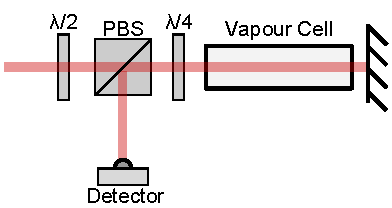
\includegraphics[width=\linewidth]{chapter1/Figs/SatAbs.pdf}
\caption{Saturated absorption spectroscopy.}
\end{figure}
\subsection{PDH}
\subsection{other modulation based techniques}
\section{Theoretical Desciption of Polarisation Spectroscopy}\label{section:pol_spec_theory}
\subsection{Basic Theory}

In \gls{ps} a circularly polarised pump beam from a monochromatic laser, with frequency close to an atomic resonance, induces frequency-dependent circular birefringence in a magnetically-shielded atomic gas sample.
A linearly polarised beam from the same source is used to measure the birefringence, monitored with a balanced polarimeter consisting of a half-wave phase retarder, \gls{pbs} and two detectors.
This is shown in Figure \ref{figure:pol_spec_schematic}.

\begin{figure}
\centering
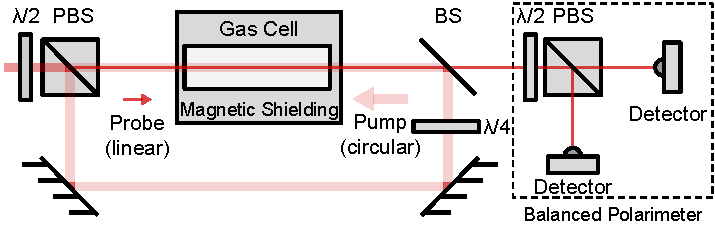
\includegraphics[width=\linewidth]{chapter1/Figs/PolSpecSchematic.pdf}
\caption{A schematic of \gls{ps} with a balanced polarimeter.
The power balance between the probe and the pump beam is controlled with the left-most $\lambda/2$ phase retarder and \gls{pbs}.
The $\lambda/4$ retarder is adjusted to produce a circularly polarised pump beam.
The non-polarising beamsplitter (BS) is used to counter-propagate the pump beam through the atomic sample without altering the polarisation of the circular pump or linear probe.
The final $\lambda/2$ retarder, \gls{pbs} and the detectors form the balanced polarimeter that monitors the polarisation rotation of the probe.}
\label{figure:pol_spec_schematic}
\end{figure}

The circularly polarised pump beam induces cicular birefringence in the atomic sample by partially optically pumping the sample into one of the extreme hyperfine sublevels, $m_F=\pm F$, where $m_F$ labels the hyperfine sublevel and $F$ labels {\color{red}some quantum thingy.}
This partial optical pumping, referred to here as the anisotropy fo the medium, results in unequal absorption coefficients for each circular polarisation.
The linearly polarised probe beam can be decomposed into two equal and oppositely circularly polarised components which undergo different absorption due to the anisotropy, such that when recombined after passing through the atomic sample the probe beam becomes elliptically polarised with an angle different to that of the original linear polarisation.
This process is depicted in Figure \ref{figure:pol_spec_explanation}.

\begin{figure}
\centering
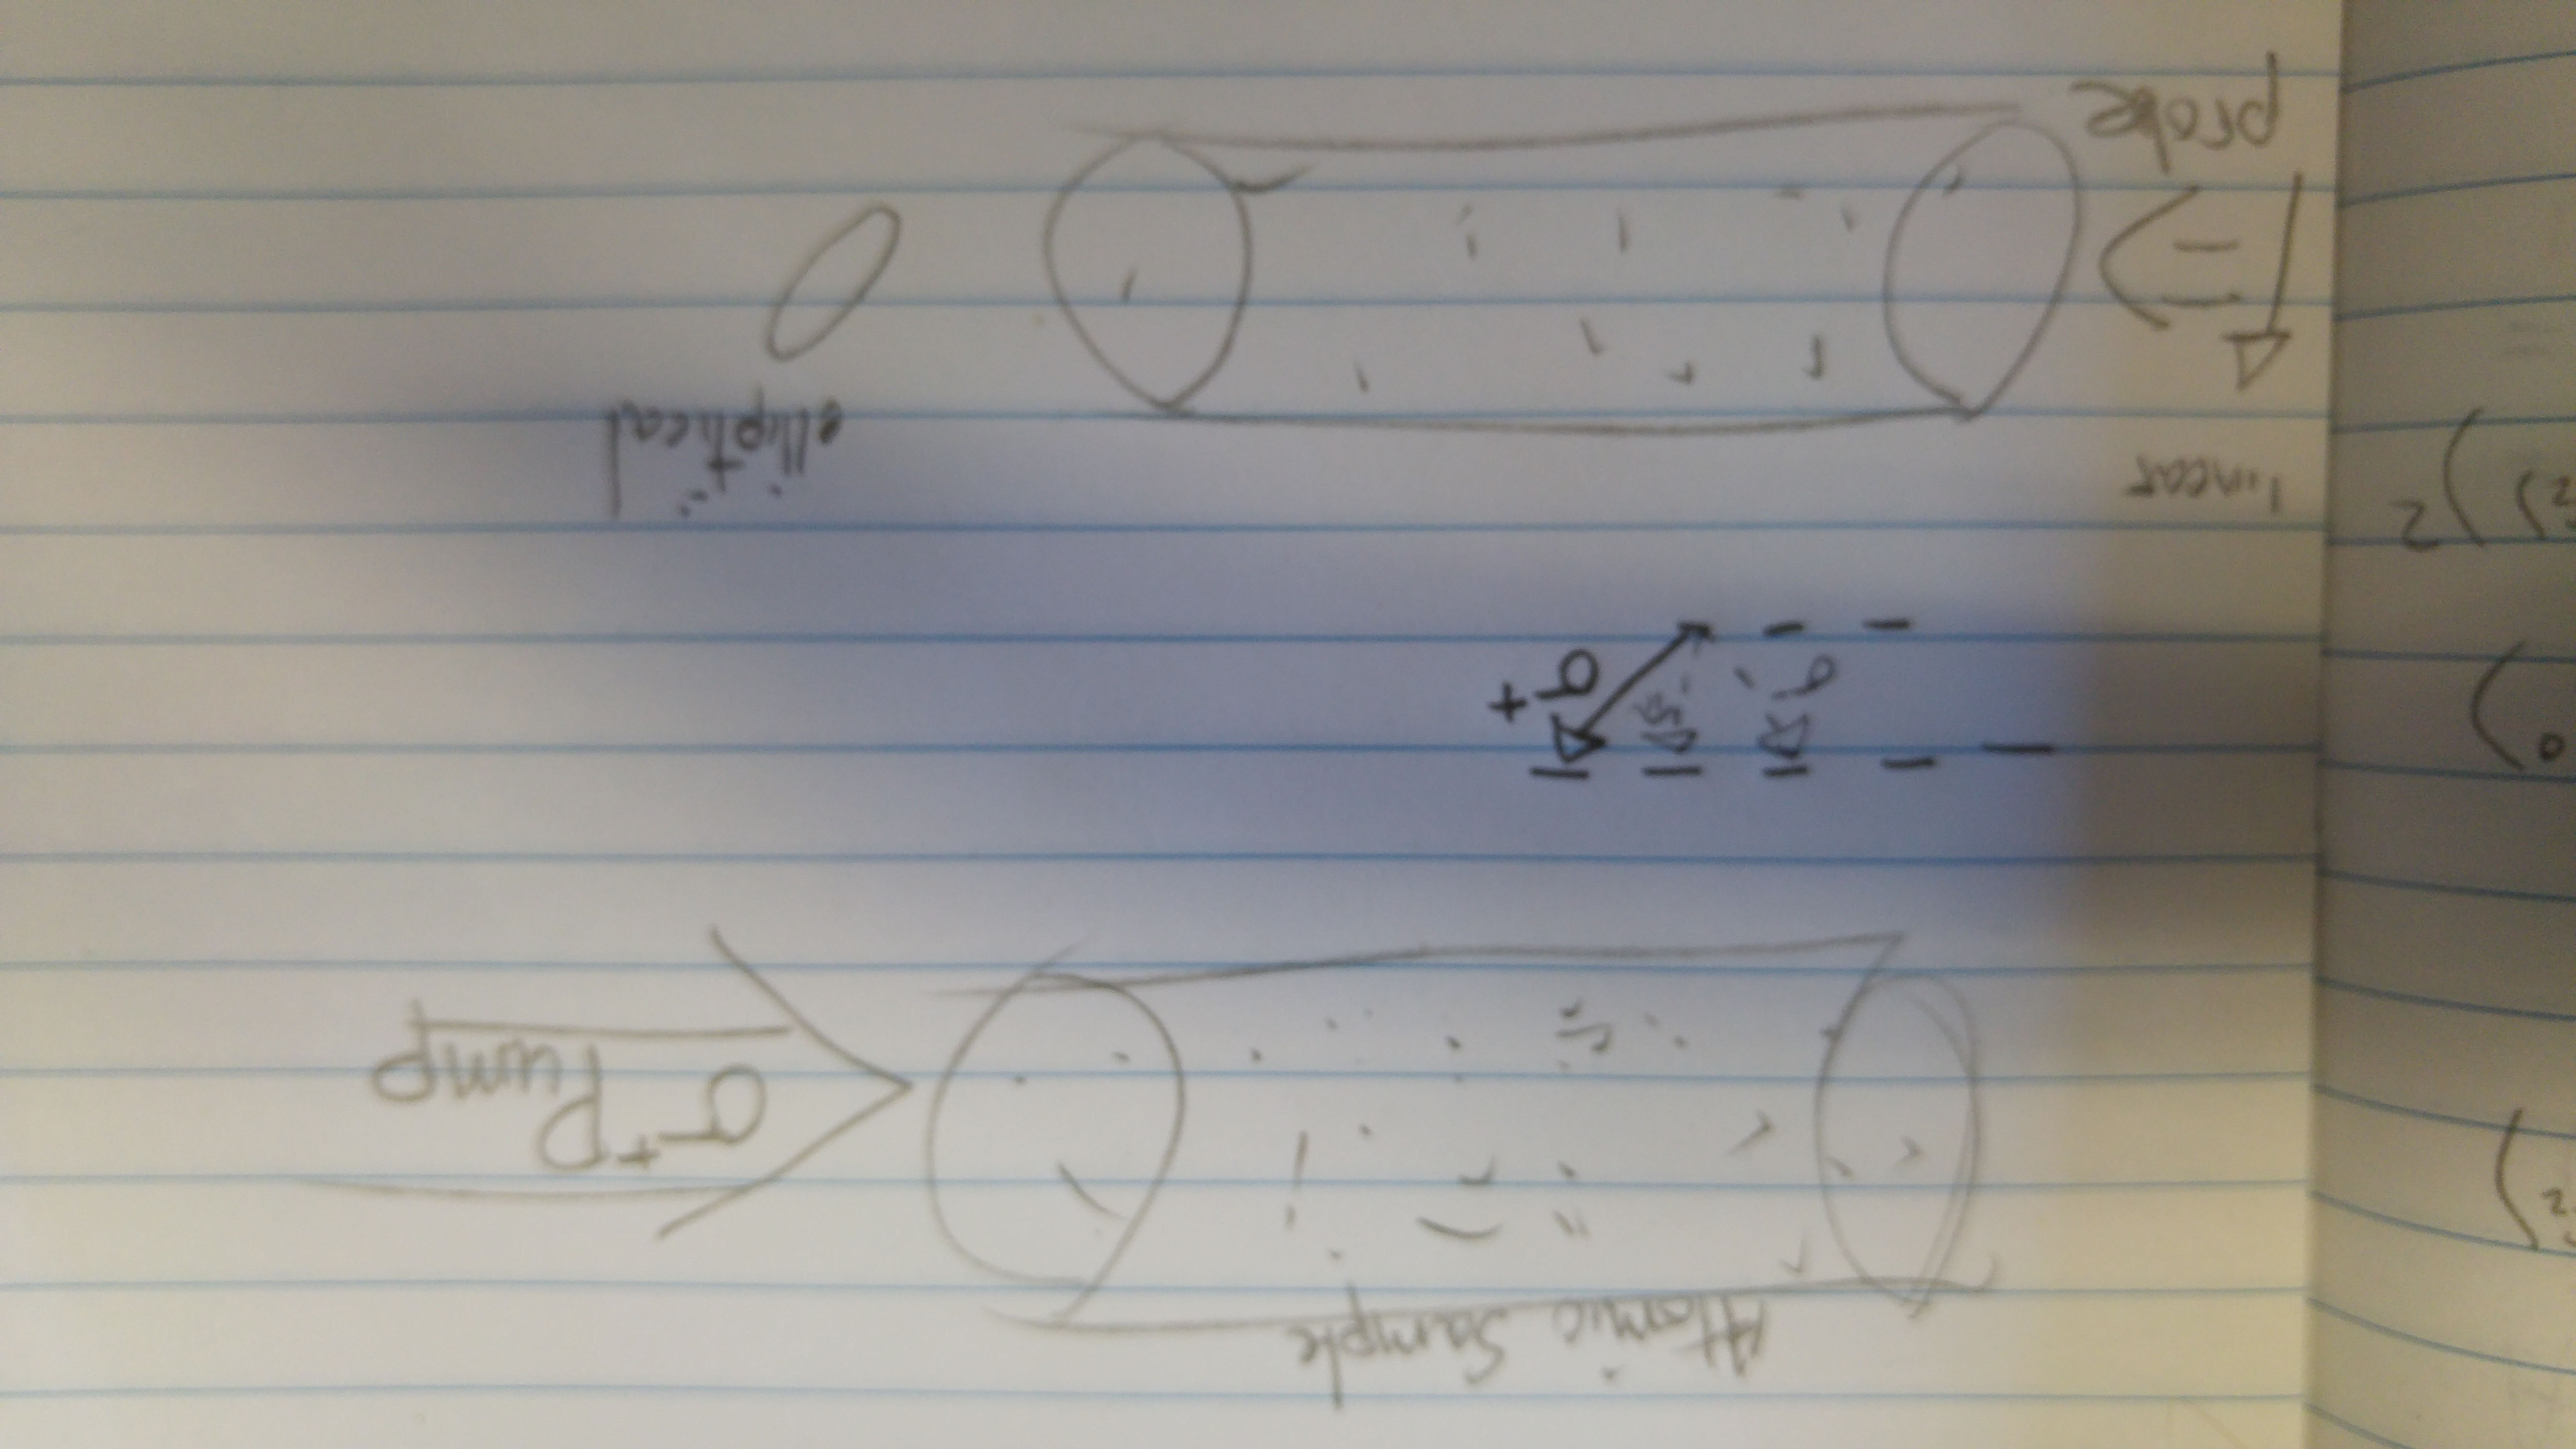
\includegraphics[width=\linewidth,angle=180]{chapter1/Figs/pol_spec_explanation_placeholder.jpg}
\caption{A conceptual figure for explaining the basics of pol spec.}
\label{figure:pol_spec_explanation}
\end{figure}

Consider the electric field of the probe beam before it enters the atomic sample at an angle $\phi$ to the $x$ axis:
\begin{equation}
\vec{E}=E_0\big(\cos{\phi}\,\hat{x}+\sin{\phi}\,\hat{y}\big)
\end{equation}
which can be expressed in terms of the circularly polarised basis vectors:
\begin{equation}
\vec{E} = \frac{E_0}{2}e^{-i\phi}(\hat{x}+i\hat{y}) + \frac{E_0}{2}e^{+i\phi}(\hat{x}-i\hat{y})
\end{equation}

After propagating through an atomic sample of length $L$ with refractive indices for the circular polarisation components of $n_\pm$, $\vec{E}$ and absorption coefficients of $\alpha_\pm$ the electric field becomes
\begin{align}
\vec{E} = &\frac{E_0}{2}e^{-i\phi}(\hat{x}+i\hat{y})\,\exp\left[\frac{i\omega n_+ L}{c} - \frac{\alpha_+ L}{2}\right] +\notag\\
&\frac{E_0}{2}e^{+i\phi}(\hat{x}-i\hat{y})\,\exp\left[\frac{i\omega n_- L}{c} - \frac{\alpha_- L}{2}\right]\label{equation:elliptically_polarised}
\end{align}

Equation \ref{equation:elliptically_polarised} represents elliptically polarised light with the major axis at an angle of $\theta$ to the $x$-axis, where
\begin{equation}
\theta = \phi + \frac{\pi L (n_+ - n_-)}{\lambda}
\end{equation}
thus the angle by which the probe has rotated is
\begin{equation}
\Phi = \frac{\pi L \Delta n}{\lambda},
\end{equation}
where $\Delta n = n_+ - n_-$.

The electric field after the sample can be approximated to {\color{red}(probably don't need to make this approximation going from 1.3 to 1.7)}
\begin{equation}
\vec{E} = E_0\big(\cos\left[\phi+\Phi\right]\,\hat{x}+\sin\left[\phi+\Phi\right]\,\hat{y}\big).
\end{equation}

The output of the balanced polarimeter is the difference between the intensity {\color{red}(? I or P?)} of light incident on each detector:
\begin{align}
I_{out} = I_x - I_y &= \frac{1}{2}\epsilon_0 c \left(|E_x|^2 - |E_y|^2\right)\notag\\
&= \frac{1}{2}\epsilon_0 c \left(\cos^2\left[\phi+\Phi\right] - \sin^2\left[\phi+\Phi\right]\right)\notag\\
&= \frac{1}{2}\epsilon_0 c \cos\left[2\phi+2\Phi\right]\notag\\
&= I_0 \cos\left[2\phi+2\Phi\right]
\end{align}

The largest spectrum is provided when $\phi=\pi/4$ and since $\Phi$ is small $I_out$ can be approximated to
\begin{equation}
I_{out} = I_0 2\Phi = I_0 \frac{2\pi L \Delta n}{\lambda}
\end{equation}

\subsubsection{Theory from paper - to be merged}
A schematic diagram for polarization spectroscopy is shown in Fig.~\ref{polspec_schematic}.
A circularly polarized pump beam from a monochromatic laser induces frequency-dependent circular birefringence in a magnetically-shielded atomic gas sample.
A linearly polarized beam from the same source is used to measure the birefringence, monitored with a balanced polarimeter consisting of a half-wave phase retarder, \glsfirst*{pbs} and two detectors.
The difference, or error, signal from the two detectors is of the form \cite{pearman_polarization_2002}
\begin{align}
P_{PS} = P_x-P_y = -P_0 \cos(2\phi+2\Phi)\label{P_PS}
\end{align}
where $P_{x,y}$ are the power of the horizontal and vertical linearly polarized components of the probe after the sample, $P_0$ is the power of the probe in the absence of a pump beam, $\phi$ is the angle of polarization of the probe in the absence of a pump beam and $\Phi$ is the additional polarization rotation of the probe due to the birefringence induced by the pump.
The largest \gls*{ps} spectrum is produced when $\phi=\pi/4$ and since $\Phi$ is small Eq.~(\ref{P_PS})  becomes
\begin{align}
P_{PS} = 2P_0 \Phi.
\end{align}
The polarization rotation is given by
\begin{align}
\Phi = \frac{\pi L \Delta n}{\lambda},
\end{align}
where $L$ is the length of the atomic sample, $\lambda$ is the wavelength of the light, $\Delta n = n_+ - n_-$ and $n_\pm$ are the refractive indices affecting the circularly polarized components of the probe beam $\sigma^\pm$.
\begin{figure}[htbp]
\centering
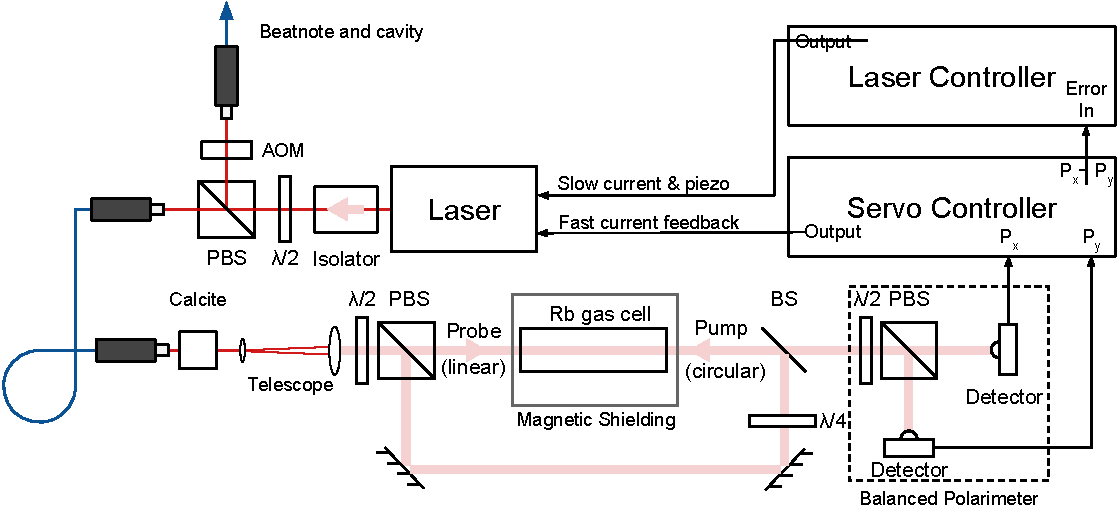
\includegraphics[width=\linewidth]{chapter1/Figs/fig1.pdf}
\caption{Schematic of a polarization spectroscopy (PS) apparatus.
The beam from the ECDL laser passes through an isolator before being split into two beams by a polarizing beam cube (PBS) and coupled into optical fibers.
One fibre leads to the PS setup and the other to other measurement or experimental apparatus.
The PS setup  consists of a polarization stabilizing calcite prism followed by a beam expanding telescope.
The expanded beam is then divided by a PBS into a linearly polarized probe and circularly polarized pump which counter-propagate, via a non-polarizing 50:50 beamsplitter (BS), through the magnetically shielded atomic gas sample.
The polarization rotation of the probe beam is then measured by a balanced polarimeter which consists of a $\lambda/2$ waveplate, PBS and two detectors.}
\label{polspec_schematic}
\end{figure}

The spectral profile of the difference in absorption coefficients for the circularly polarized components for the atomic medium in the vicinity of a resonance is a Lorentzian with width $\Gamma$, the inverse lifetime of the excited state of the resonant transition~\cite{demtroder_laser_2003}:
\begin{align}
\Delta \alpha = \frac{\Delta\alpha_0}{1+4\left(\frac{\delta}{\Gamma}\right)^2}.
\end{align}
Here $\delta=\omega_L-\omega_A$ is the detuning of the laser from the resonance, $\omega_L$ is the angular frequency of the laser and $\omega_A$ the angular frequency of the atomic resonance.
$\Delta\alpha_0$ is the difference in absorption coefficients for the $\sigma^\pm$ circular polarization components at zero detuning.

The refractive index and absorption of the medium are related through the Kramers-Kronig dispersion relation \cite{demtroder_laser_2003},
\begin{align}
\Delta n = \Delta\alpha_0 \frac{2c}{\omega_A \Gamma}\frac{\delta}{1+4\left(\frac{\delta}{\Gamma}\right)^2}.\label{result}
\end{align}
$\Delta\alpha_0$ is the sum over all $m_F$ ground states of the difference between absorption coefficients for each circular polarization, with $\delta=0$, weighted by the ground ($F, m_F$) and excited state ($F', m_{F\pm1}$) population differences,
\begin{align}
\Delta\alpha_0 = \sum_{m_F=-F}^{+F} \big[\alpha_{(F,m_F\rightarrow F',m_{F+1})}(P_{F,m_F}-P'_{F',m_{F+1}})\nonumber\\
-\alpha_{(F,m_F\rightarrow F',m_{F-1})}(P_{F,m_F}-P'_{F',m_{F-1}})\big].
\end{align}
The absorption coefficient for a given transition is $\alpha_{(F, m_F\rightarrow F',m_{F\pm1})}=N \sigma(\omega_L)$ where $N$ is the total number of interacting atoms, $\sigma(\omega_L)$ is the absorption cross section for the transition and $P_{F,m_F}$ refer to the populations of the various atomic states.

\subsubsection{Magnetic shielding}

\subsection{Fast Theory}

\subsubsection{from paper}
The atomic substate populations can be calculated using \glspl*{obe}~\cite{hughes_polarization_2009} but the standard steady-state solutions provide little insight into the behavior of the error signal when $\delta$ is changing faster than the evolution of the populations.
That evolution is limited to the spontaneous decay rate $\Gamma$, and hence for times $t\ll \tau=1/\Gamma$, the populations can be considered constant.
The \gls*{ps} signal is proportional to the refractive index difference given by Eq.~(\ref{result}), which describes a steep, background-free antisymmetric dispersive function, with bandwidth $1/t$ that can be much greater than $\Gamma$ (Fig.~\ref{sa_ps_spectra}).
Absorption-based frequency stabilization techniques such as \gls*{sa} rely on frequency-dependent changes to the atomic populations, rather than on the refractive index, resulting in dispersive signals over a much smaller capture range, with bandwidth limited to $\Gamma$.
SA is further limited if there are closely spaced hyperfine resonances or cross-over peaks.
Laser frequency noise can extend to frequencies much greater than $\Gamma$, where polarization spectroscopy still provides strong feedback and therefore can achieve much narrower laser linewidth.

\subsection{OBEs (timescale of state evolution, step in simulating)}
\section{Developments}
\subsection{Balanced Polarimeter}
When Wieman and H\"anch~\cite{wieman_doppler-free_1976} originally described \gls{ps} polarisation rotation was monitored with a nearly crossed polariser as shown in Figure \ref{figure:wieman_doppler-free_schematic}.
The polariser is crossed such that only a small proportion of the probe beam passes through them in the absence of the pump.
With the pump inducing anisotropy the rotation of the probe can be detected after the polarisers.

\begin{figure}
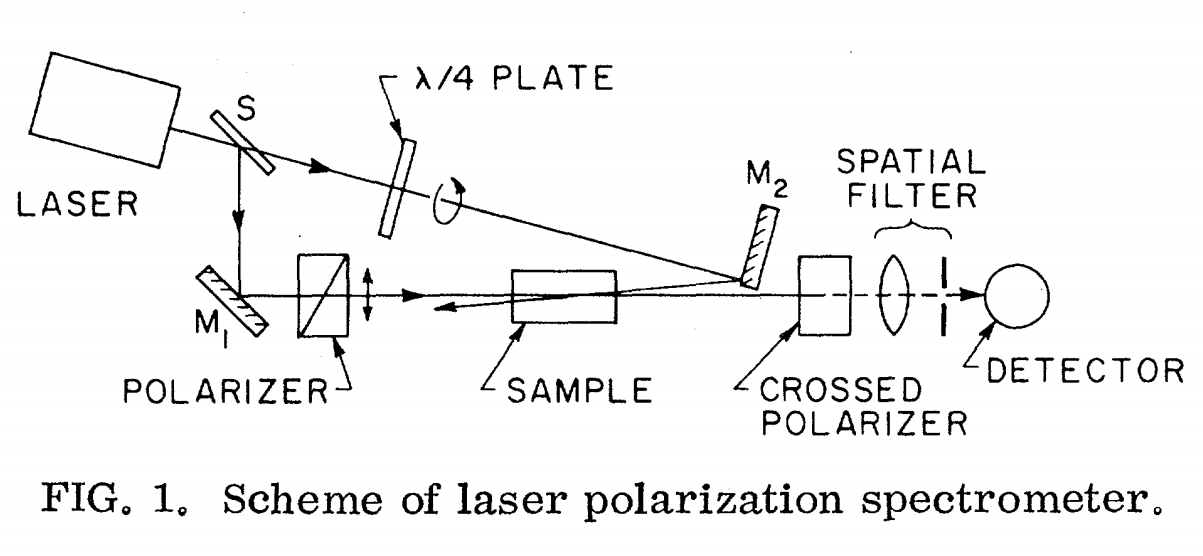
\includegraphics[width=\linewidth]{chapter1/Figs/wieman_doppler-free_schematic.png}
\caption{Figure stolen from Wieman and H\"anch paper.
Should probably redraw so I'm not plagiarising.
Or ask how to cite it probably or some such.}
\label{figure:wieman_doppler-free_schematic}
\end{figure}

Pearson et al. proposed the alternative method of using a balanced polarimeter which provides a background-free signal with peak-to-peak height more than an order of magnitude greater than with the crossed polariser method~\cite{pearman_polarization_2002}.

\subsection{Beam splitter to co-propagate}

All papers thus far have ``snuck'' the pump beam through the vapour cell.

Figure with ``snucked'' and beam splitter configuration.

The angle of ``snucking'' has implications that there is math for...

Using a NBPS instead means you have an angle of 0.
The beam splitter has no effect on the polarisation as far as I can tell.

Pumped spectrsocopy techniques such as \gls{ps} and \gls{sa}... spectral broadening due to angle stuff.

\subsection{High bandwidth feedback}


\subsection{Lincoln's magic detectors?}
\section{Experimental Setup (with details - fibres, calcite, etc.)}
\subsection{from paper - merge}
Two commercial Littrow configuration \glspl*{ecdl} \cite{equipment} were individually locked using \gls*{ps}.
The laser beam for each was split by a \gls*{pbs} and propagated through polarization-maintaining fibers to the \gls*{ps} locking system and linewidth measurements.
The locking beams were polarized with Glan-Thompson prisms (Fig.~\ref{polspec_schematic}) to eliminate residual polarization drift in the fibers.
Beam expanding telescopes were used to expand the beam to fill the apertures of the magnetic shielding, approximately 1\,cm diameter, allowing them to interact with more atoms to increase $|\Delta\alpha_0|$ and improve the \gls*{snr}.

The \gls*{pbs} balanced polarimeter error signal was generated with biased photodiodes (150\,MHz bandwidth) and servo controllers (14\,MHz bandwidth).
The servo controller integration zero-gain frequency was typically between 100\,kHz and 1\,MHz.
The diode modulation could be DC-coupled, with bandwidths of 40\,MHz and 10\,MHz, or AC-coupled, 100\,kHz\,\textendash\,40\,MHz and 10\,kHz\,\textendash\,10\,MHz, depending on the laser.
The laser electronics provided control of the \glspl*{ecdl} piezoelectric transducer and diode injection current, with bandwidths of 1\,kHz and 50\,kHz respectively.

\section{Measurement Techniques}
We have characterized the performance of \gls*{ps} locking by measuring the noise-limited bandwidth of the error signal, the spectral linewidth of the locked lasers using high-finesse optical cavity transmission and heterodyne techniques, the frequency noise spectra of the locked lasers, and the long-term frequency stability of the locked lasers.

\subsection{Self-heterodyne}

Self-heterodyne is...

Single delay...

How much delay?

Multipass delay...

These are the results I got...

They look good... too good.

Here's why...\cite{richter_linewidth_1986}

\subsection{Heterodyne}
\subsubsection{from paper - merge}
To investigate the discrepancy between the two laser linewidth measurements we used heterodyne measurements which are insensitive to amplitude noise.
Heterodyne measurements were made by frequency shifting one of the laser beams with a double-pass \gls*{aom} and combining the two locked beams on a 50:50 beamsplitter followed by a 1\,GHz bandwidth photodetector.
The beatnote spectrum was measured with a radio frequency spectrum analyzer~\cite{equipment}, see Fig.~\ref{beatnote}.
Most of the optical power is within the central peak of the spectrum, with $-3\rm\,dB$ full width of $2.0\pm1.1$\,kHz determined from a Gaussian fit.
The lasers are uncorrelated and if they have identical, Gaussian lineshapes then the single laser \gls*{rms} linewidth is $0.60\pm0.32$\,kHz.
The shoulders in the spectrum around $\pm1.5$\,MHz correspond to the servo bump of the fully locked spectra in Fig.~\ref{fig:PSDs}.

{\color{red} Rob to determine single laser linewidth from -3dB beatnote width}

\begin{figure}[htbp]
\centering
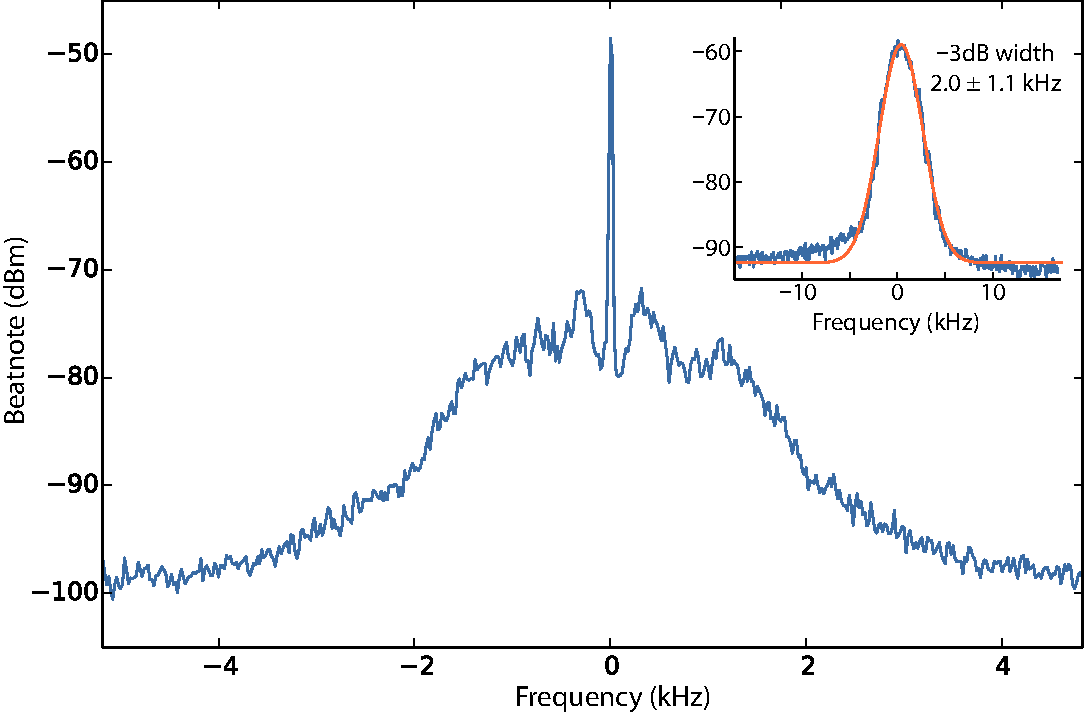
\includegraphics[width=\linewidth]{chapter1/Figs/fig5_v1.pdf}
\caption{Heterodyne beatnote for the two lasers locked with \gls*{ps}.
The inset figure is a higher resolution measurement of the central peak with a Gaussian fit (red), $-3\rm\,dB$ width of 2.0$\pm$1.1\,kHz.
Both figures are 50 shot averages with resolution bandwidths of 30\,kHz and 100\,Hz and total measurement times of approximately 0.5\,s and 2\,s respectively.}
\label{beatnote}
\end{figure}

\begin{table}[htbp]
\centering
\begin{tabular}{c c c}
\hline
  & Method & RMS Linewidth (kHz) \\ \hline
  (i) & Cavity transmission mapping  & $2.0 \pm 0.4$ \\
  (ii) &Cavity transmission integral & $2.4 \pm 1.0$ \\
  (iii) & Heterodyne & $0.60\pm0.32$ \\ \hline\end{tabular}
\caption{Linewidth results.
(i) Mapping the transmission signal through a cavity with a \gls*{fwhm} of 71.6\,kHz to a Lorentzian signal followed by deconvolving from the amplitude noise.
(ii) The results from integrating the power-spectral density of the cavity transmission signal (Fig.~\ref{fig:PSDs}) (iii) The heterodyne beatnote (Fig.~\ref{beatnote}).}
\label{linewidth_table}
\end{table}

\subsection{Noise measurements}
\subsubsection{From paper - merge}
\begin{figure}[htbp]
\centering
    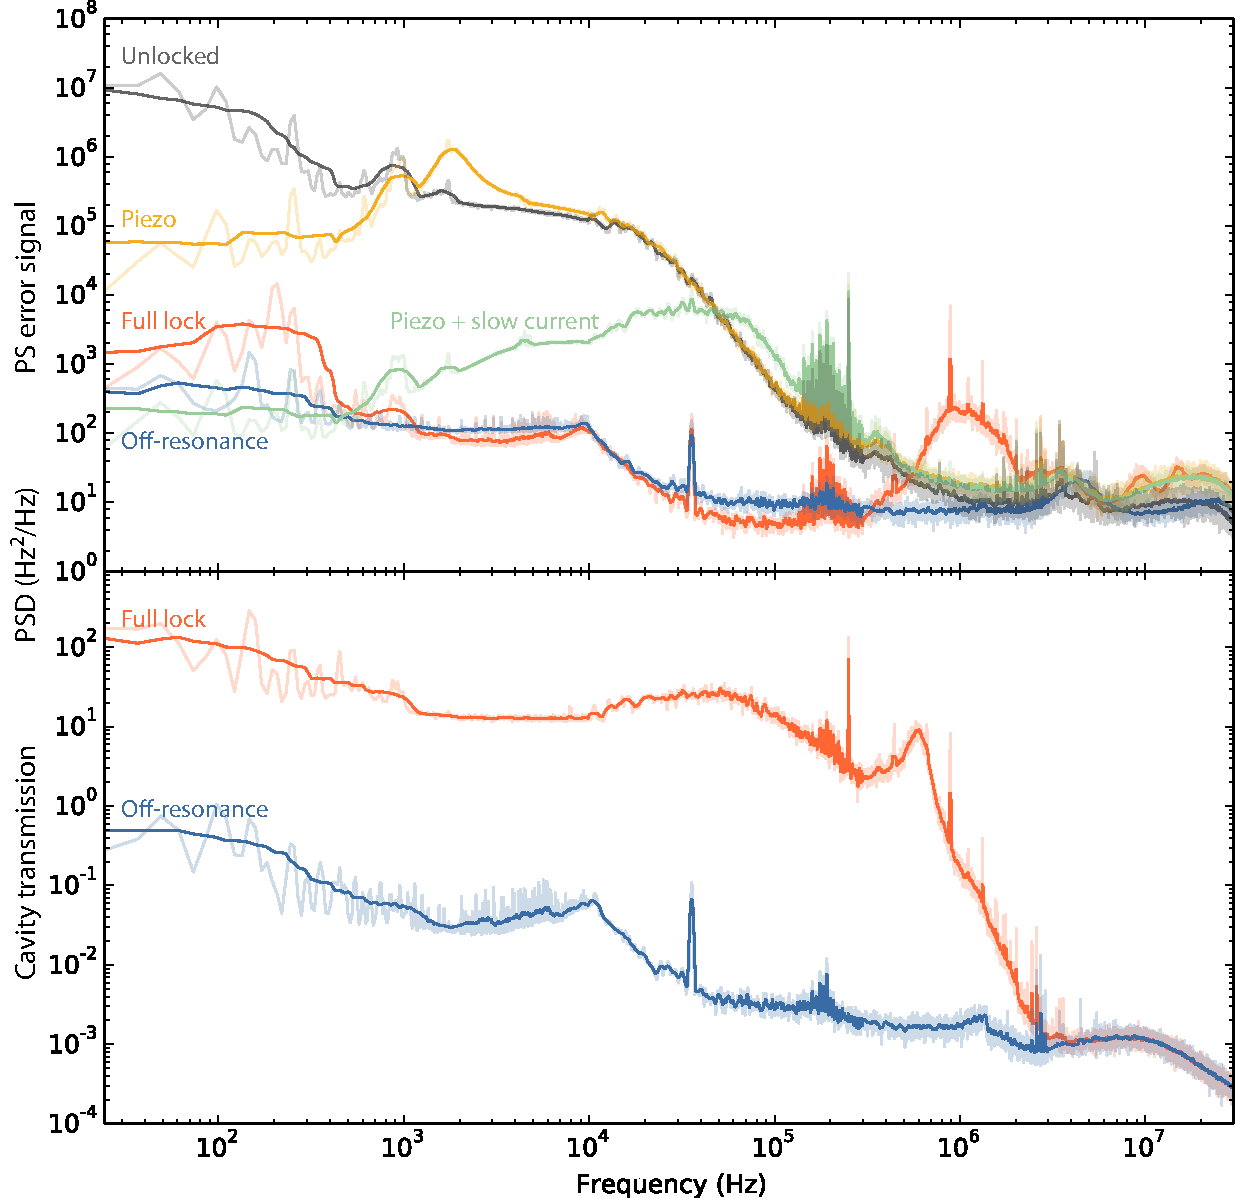
\includegraphics[width=0.9\linewidth]{chapter1/Figs/fig4a_v3.pdf}
    \label{fig:PSDs}
    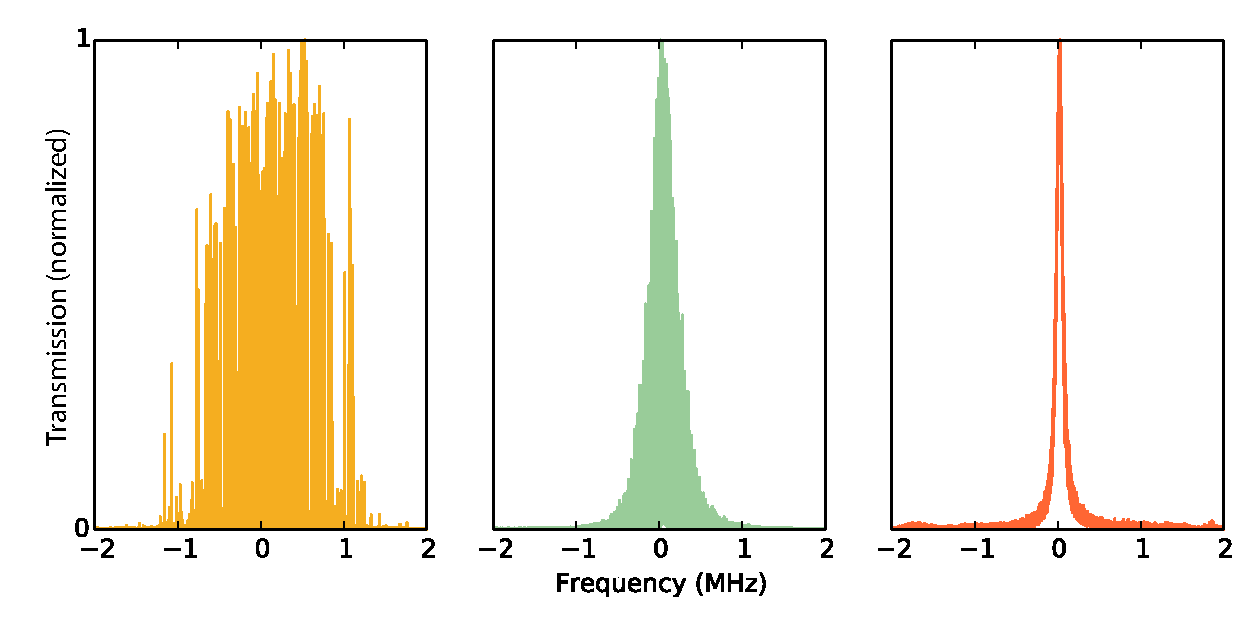
\includegraphics[width=0.9\linewidth]{chapter1/Figs/fig4b_v1.pdf}
    \label{fig:cavity_scans}
\caption{Frequency noise measurements.
(a) \Gls*{psd} of polarization spectroscopy error signals for a range of laser locking regimes with laser on resonance: unlocked; piezo-only feedback; slow current and piezo feedback; piezo, slow current, and fast AC-coupled current feedback; the noise floor of the noise measurement with no light on the \gls*{ps} detectors.
Laser power 6.5\,mW.
The measurements are shown with a superposed smoothed curve (moving average  with window size $10\log_{10}(f)$ where $f$ is the frequency).
(b) Optical cavity transmission as a function of laser offset frequency for locking with varying bandwidth.
Piezo only (left), piezo and slow current (middle) and piezo, slow current and fast current (right).
Cavity \gls*{fwhm} linewidth 71.6\,kHz, scan time 100\,ms, laser power $170\rm\,\mu W$.
(c) \Gls*{psd} of transmitted cavity signal at half peak height for the piezo, slow current and fast AC-coupled current feedback.
For (a) and (c) noise below $10^4$\,Hz was measured with a high dynamic range audio digitizer with a resolution bandwidth (RBW) of 12\,Hz; an RF spectrum analyzer was used at higher frequencies, with RBW of 30\,Hz between $10^4$\,Hz \textendash$10^6$\,Hz and RBW of 300\,Hz above $10^6$\,Hz.} 
\end{figure}

\subsubsection{Error Signal Noise}
The spectrum of the \gls*{ps} error signal provides a measure of the laser frequency noise in combination with the \gls*{ps} frequency discrimination, photodetector and electronic noise and gain.
The response of the system to different feedback parameters and the underlying noise limitations are immediately apparent.
The frequency noise \glsfirst*{psd} of the \gls*{ps} error signal (Fig.~\ref{fig:PSDs}) was measured for different feedback configurations, using a high-dynamic-range audio digitizer (low frequency, \textless10\,kHz) and radio-frequency spectrum analyzer (high frequency, 10\,kHz to 30\,MHz).
The spectrum analyzer was calibrated using the slope of the error signal at resonance.
The low frequency data were calibrated by matching to the spectrum analyzer data at 10\,kHz.  

Increasing suppression of noise is readily apparent as the feedback bandwidth is increased from 1\,kHz (piezo only) to 50\,kHz (piezo and slow current through the laser controller) and then full lock with feedback via direct diode current modulation.
From around 450\,Hz to 350\,kHz the fully locked noise spectrum is coincident with the noise floor measured by detuning the laser far from resonance, and intersects with the unlocked spectrum at 700\,kHz.
A servo bump peaked at 1.3\,MHz is consistent with a phase lag in laser diode response to current modulation \cite{wiemanhollberg}.

%{\color{red} Need to say ``so what''.   The data show feedback signal of 15 to 20\,dB above noise, over a bandwidth limited by the servo controller bandwidth of 14\,MHz. [Comment applies to Fig.2?] Useful feedback to about 700\,kHz, lower than SNR bandwidth of about 2\,MHz due to diode phase lag. }

%{\color{red} Explain why bandwidth appears to be so much less than Fig.2? Actually it's not but Fig 2 shows 0.1 - 100 MHz?}

\subsubsection{Cavity Transmission Noise}
The error signal spectra provide useful information for optimising the locking system to reduce the laser frequency noise spectrum.
To measure the laser frequency noise spectrum itself we used a high-finesse optical cavity as an independent laser frequency discriminator \cite{equipment}.
With finesse of 20942 and free spectral range of 1.50\,GHz, the optical cavity had \gls*{fwhm} linewidth of 71.6\,kHz. 
Fig.~\ref{fig:cavity_scans} shows cavity transmission signals as the laser frequency incident on the cavity was scanned with a double-pass \gls*{aom}.
The resulting traces provide a clear illustration of the effect of increased locking bandwidth: with piezo-only locking the peak appears broad as the laser jitters around the resonant frequency.
With slow current feedback, the transmission peak shape becomes apparent, and finally we see the effect of high-bandwidth feedback with peak width limited by the cavity finesse, indicating a laser linewidth much smaller than the cavity linewidth.

We analyzed the frequency noise of the laser through the cavity transmission signal by choosing a static \gls*{aom} frequency such that the transmitted power through the optical cavity was half the peak power, where the transmission-frequency response is approximately linear. 

The cavity noise spectrum is shown in the lower portion of Fig.~\ref{fig:PSDs} for full bandwidth AC-coupled locking.
The signal was well above the noise floor, measured with laser frequency between transmission peaks, for frequencies up to the 5.5\,MHz bandwidth of the photodetector.
 This approach could not be used with lower-bandwidth feedback because the laser linewidth was wider than the cavity transmission.
 Note that the cavity transmission noise floor is three to four orders of magnitude lower than that of the \gls*{ps} error signal, in part due to the much lower laser power (microwatts rather than milliwatts) and hence lower shot noise.

We extracted a measure of the linewidth from the cavity data using two methods: first we mapped the amplitude noise of the locked cavity signal to frequency using the cavity transmission frequency response shown in Fig.~\ref{fig:cavity_scans}.
The standard deviation of the distribution of frequencies gave an \gls*{rms} linewidth of 2.4$\pm$0.4\,kHz.
We also integrated the power spectral density to find an RMS linewidth \cite{negnevitsky_wideband_2013} of 2.4$\pm$1.0\,kHz.
Linewidth results are summarized in Table \ref{linewidth_table}.

The cavity transmission spectra and linewidth measurements include contributions from both laser frequency and amplitude noise.
An estimate of the amplitude noise contribution to the spectra was obtained by measuring the photodetector power spectrum without the cavity and thus without frequency noise, with the same incident laser power on the photodetector.
Mapping that noise spectrum to frequency produced a contribution of 1.4$\pm$0.3\,kHz in the cavity transmission mapping linewidth,  and 0.16$\pm$0.07\,kHz to the PSD integral linewidth.
As expected, the cavity transmission mapping method is more susceptible to laser amplitude noise. 

Assuming the measurements are uncorrelated convolutions of the frequency and amplitude noise contributions, the linewidth determined from cavity transmission mapping consists of the 1.4$\pm$0.3\,kHz amplitude noise linewidth in combination with a frequency noise linewidth of 2.0$\pm$0.7\,kHz.
The difference is likely because the mapping method does not properly include contributions from higher Fourier frequencies; that is, the ``pedestal'' of the laser spectrum which can be seen in a heterodyne measurement.

\subsection{Side of peak (include basic cavity theory here?)}
\subsection{Integration}
\subsection{Drift}
\subsection{Bandwidth Stuff}
\subsubsection{From paper - merge}
\label{bandwidth_section}
The capture range and bandwidth of the frequency discriminator are important in determining the ultimate linewidth that can be achieved, and the ability to compensate for sudden disturbances to the laser frequency, for example due to external shock or vibration.
We define the capture range as twice the minimum frequency difference from resonance for which the locking signal is of the correct sign for negative feedback, which can be deduced from the error signal by locating the first zero crossing to either side of the resonance.
For the spectra shown in Fig.~\ref{sa_ps_spectra} this is greater than $300\rm\,MHz$, many times larger than the $16\rm\,MHz$ of \gls*{sa}, as shown in Fig.~\ref{sa_ps_spectra}.

The frequency noise spectrum of the \gls*{ps} error signal is shown in  Fig.~\ref{bandwidth}, both on-resonance and with laser far detuned to determine the noise floor.  The signal and noise intersect at 83\,MHz.
Since the sign of the \gls*{ps} error signal is constant over that range (see fig.~\ref{sa_ps_spectra}), the 83\,MHz noise-limited signal bandwidth is indicative of the high bandwidth available from polarization spectroscopy.
In contrast, the \gls*{sa} signal reverses sign several times within 83\,MHz, and the effective bandwidth is limited by the $\pm 8\rm\,MHz$ capture range of \gls*{sa}.

\begin{figure}[htbp]
    \centering
    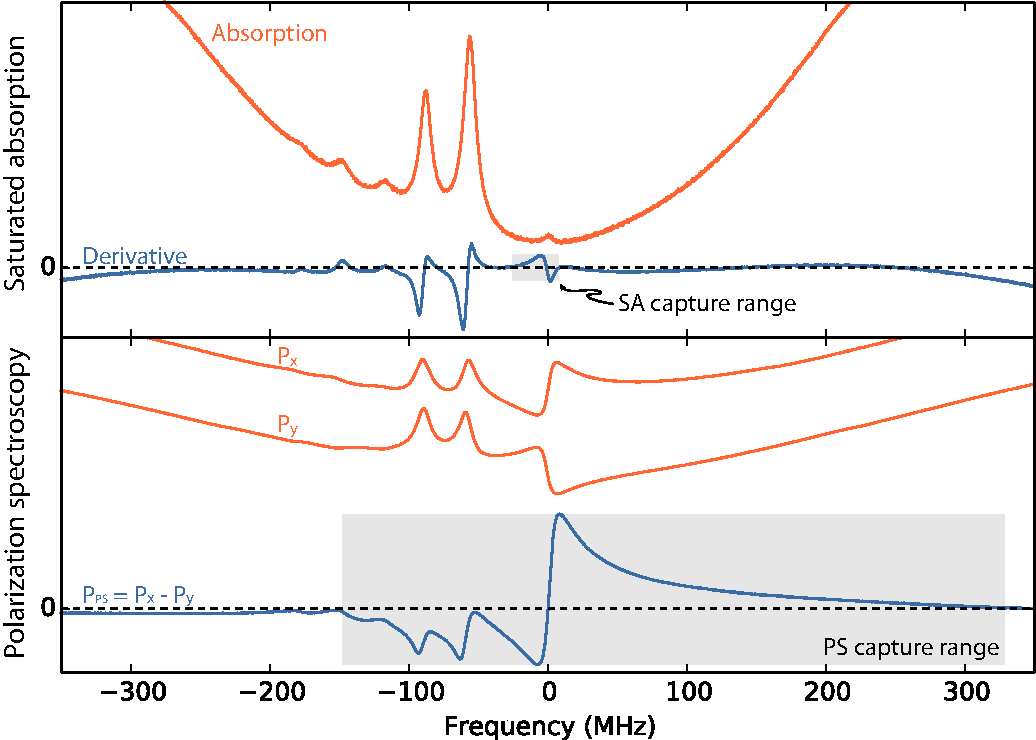
\includegraphics[width=\linewidth]{chapter1/Figs/fig2_v1.pdf}
    \caption{Saturated absorption spectroscopy (SA) and polarization spectroscopy (PS) spectra for the $^{85}$Rb D2 transition.
The upper portion of the figure shows the absorption and error spectra for SA.
The lower portion shows the components of the PS error signal ($P_{x,y}$ in Fig. \ref{polspec_schematic} and Eq. \ref{P_PS}) and the PS error signal.
The shaded regions indicate the approximate capture range of the respective error signals.
Zero frequency at $^{85}$Rb, $5^2S_{1/2} F=3\rightarrow5^2P_{3/2} F=4$ transition.
Absorption signals normalized to the same maximum absorption on resonance.}
    \label{sa_ps_spectra}
\end{figure}

\begin{figure}[hbp]
    \centering
    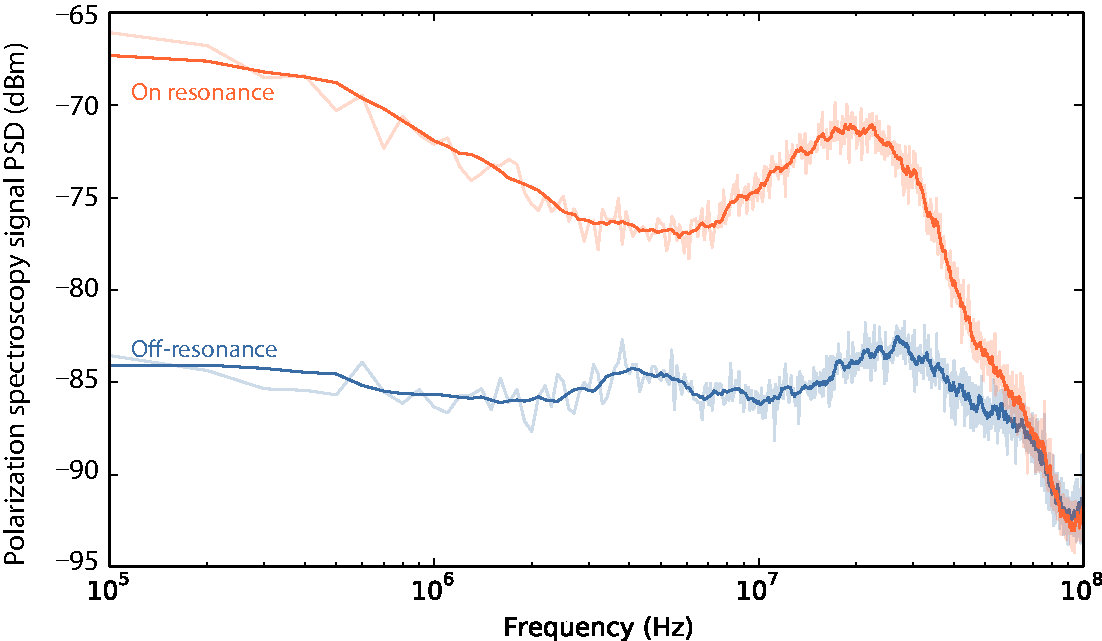
\includegraphics[width=\linewidth]{chapter1/Figs/fig3_v1.pdf}
    \caption{Polarization spectroscopy error signal frequency noise spectra.
Upper trace (black): frequency spectrum of the error signal while the laser is unlocked and centered on the $^{85}$Rb 5$^\text{2}$S$_\text{1/2}$ $\rightarrow$ 5$^\text{2}$P$_\text{3/2}$ transition.
Lower trace (red): spectrum with laser far from resonance.
The two lines intersect at approximately 83\,MHz.
Laser power 7.5\,mW after isolator, with pump:probe ratio 1.4.
The measurements are shown with a superposed smoothed curve (moving 20-point average).}
    \label{bandwidth}
\end{figure}

\subsection{Long Term Stability}
\subsubsection{from paper - merge}
Polarization spectroscopy is inherently a DC technique, susceptible to low frequency drift ($1/f$ noise), for example drift in the laser power output as the laser alignment drifts, variations in fiber coupling efficiency, variations in the atomic vapor density due to changes in temperature or local magnetic field, or changes to the electronic gains and offsets.
To quantify the long-term stability, the beatnote between a \gls*{ps}-locked laser and a laser locked to an \gls*{sa} peak was tracked over a number of days.
The \gls*{sa} laser was AC-locked using FM demodulation; that is, with current modulation at 250\,kHz and demodulation of the detected signal.
FM modulation is inherently insensitive to many of the slow variations that can affect the lock frequency, so that variations in the beatnote frequency can be attributed to the drift in the \gls*{ps} laser.
A linear fit to the beatnote data (Fig.~\ref{drift}) sets an upper limit on the frequency drift of less than 2\,kHz/h. 

Others have measured drifts of 17\,kHz/h to 1\,MHz/h~\cite{yoshikawa_frequency_2003, tiwari_laser_2006} and standard deviation of 400\,kHz \cite{lee_frequency_2014}, depending on the extent to which the apparatus was isolated from ambient temperature variation.
In our system the lasers are temperature stabilized and isolated from the environment with acrylic boxes, but the \gls*{ps} and \gls*{sa} components were not temperature controlled or shielded from the general laboratory environment.
Polarization and power stabilization of the laser, and temperature stabilization of the atomic vapor cell, are likely to improve the locking stability and drift.

\begin{figure}[htbp]
\centering
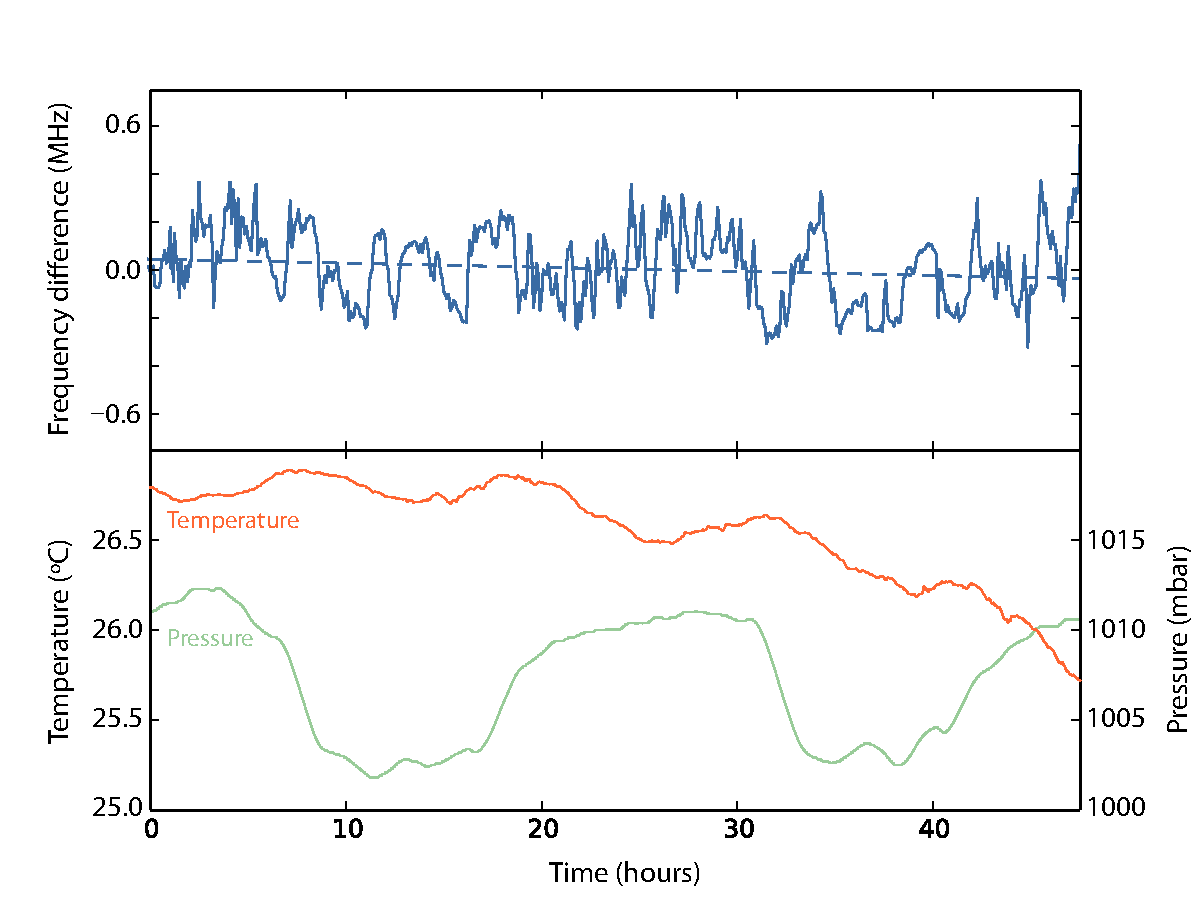
\includegraphics[width=\linewidth]{chapter1/Figs/fig6_v1.pdf}
\caption{Measurement of frequency drift of a polarization spectroscopy locked laser over a 50 hour period.
Upper: frequency deviation and linear fit with gradient -1.7\,kHz/hour sets an upper limit to the drift.
The standard deviation of the frequency measurements, acquired at 5\,min intervals, was 155\,kHz.
Lower: temperature (dotted line) and pressure (dashed line) of the laboratory over the same period of time, measured every 200\,ms.}
\label{drift}
\end{figure}

\section{Conclusion}
We have demonstrated laser frequency stabilization using a polarization spectroscopy reference, and reduced the linewidth of \gls*{ecdl} lasers well below 1\,kHz, much lower than previously demonstrated with this technique and previously achieved only by locking to high-finesse optical cavities.
The absolute frequency drift of less than 50\,kHz per day is adequate for many laser cooling experiments.
Further improvements to drift could be achieved with simple measures such as temperature stabilization and environmental isolation.
The experimental setup provides an approach with low complexity and low cost, providing wide bandwidth linewidth narrowing without radio frequency modulation while retaining an absolute atomic reference.

In our experiments, the locking bandwidth is limited by the phase lag in the laser diode response to injection current variation, to around 700\,kHz.
With appropriate servo loop shaping, for example multiple phase lead stages to compensate for the diode response, it is reasonable to expect a bandwidth increase to several MHz.
However, the effect on linewidth would be negligible because the \gls*{ps} signal-to-noise ratio is small in this frequency range.
Much greater improvements could be made by lowering the \gls*{ps} noise floor, which is three to four orders of magnitude higher than the noise floor of the optical cavity.
The difference is only partly due to the $100\times$ higher power in \gls*{ps}, which will increase shot and Johnson noise by $10\times$.
 More...
